% !TEX root = ../thesis.tex

\chapter{Preliminaries}
This is an introduction...

\section{Multi Armed Bandits}
Consider a situation in which a gambler (the \emph{agent}) is sitting in a casino, staring at a certain number of slot machines from which he wants to pick the most profitable one and play with it all night long. Each slot machine is characterized by a certain \emph{mean reward}. The objective of the gambler is to maximize the gains that he will have won by the end of the night, but, unfortunately, he can not know \emph{a priori} the mean reward associated to each slot machine. Hence, the gambler must find a suitable strategy in order to effectively \emph{explore} his possibilities, by testing the different slot machines, and, then, \emph{exploit} the ones that prove to be more profitable. In fact, the gambler would face an equivalent problem if he was to play a single machine with as many \emph{arms} (levers) as the number of slot machines present in the casino, each with its own specific mean reward. Hence the name \gls{MAB} \cite{lai1985asymptotically}, in homage to the one-armed bandit, an old-fashioned name for a lever operated slot machine ("bandit" because it steals your money). Of course, \gls{MAB}s have other, more valuable, applications other than gambling. Current applications span from web interfaces configuration, news recommendation, dynamic pricing, ad placement, networking routing and game design. 

\begin{definition} \emph{(Multi Armed Bandit)}
A \gls{MAB} is a tuple $\langle\mathcal{X}, \Rew\rangle$, where:
\begin{enumerate}
\item $\mathcal{X}$ is the $d_{\mathcal{X}}$-dimensional set of possible arms, or actions that the agent can pick; $\mathcal{X}$ can be discrete or continuous, one dimensional or multi-dimensional, finite or infinite; 
\item $\Rew:\mathcal{X}\to\Delta([-\Rmax,\Rmax])$ is an unknown function of rewards such that for every $x\in\mathcal{X}$ it assigns a probability measure $\Rew(\cdot|x)$ over $[-\Rmax,\Rmax]$, a bounded set of real-valued rewards. $\Rmax$ is the maximum absolute reward that the agent can receive.
\end{enumerate}
\end{definition}

One can think to the set of possible arms and reward functions associated to them as the \emph{environment} the learner interacts with. According to the specific characteristics of the environment, there exist a broad taxonomy of \gls{MAB}s that goes out of the scope of this work. For the reader, it is sufficient to know that in this work we deal with \emph{stochastic stationary bandits}. In this case, the environment is restricted to generate the reward in response to each action from a \emph{probability distribution} $\Rew(\cdot|x)$ that is specific to that action, stationary along time and independent of the previous action choices and rewards. For example, the reward distribution could be Gaussian or Bernoulli. The expected reward of the stationary distribution associated to arm $x$ is noted $\mu(x) = \Expu{r\sim\Rew(\cdot|x)}[r]$. \\
The \gls{MAB} game is played sequentially by a \emph{learner} over multiple rounds $t=1, 2, \dots, T$, up to the \emph{horizon} $T\in\Naturals$. Evidently, the agent can have memory but can not foresee the future. Thus, the current action $x_t$ should only depend upon the sequence of previous actions and rewards, the \emph{history} $\mathcal{I} = \{x_0, r_0, x_1, r_1, \dots, x_{t-1}, r_{t-1}\}$. A \emph{policy} is a mapping from histories to actions which represents the behaviour of the agent, its strategy. \\
the first question which springs to mind is then: how can we evaluate the quality of a policy? To this aim, the literature extensively adopts a performance measure called the \emph{regret};

\begin{definition}\label{def:immediateregret} \emph{(Immediate Regret)}
The immediate regret suffered by a learner at round $t$ is:
\begin{equation} 
\Delta_t = \mu(x^*) - \mu(x_t)
\end{equation}
where $x^* = \arg\max_{x\in\Xspace}\mu(x)$ is the arm with the highest expected reward \ie the optimal arm.
\end{definition}
\begin{definition}\label{def:regret} \emph{(Regret)}
The regret of a learner is the cumulated sum of the instantaneous regrets:
\begin{equation}
Regret(T) = \sum_{t=0}^T\Delta_t
\end{equation}
\end{definition}

The quality of a certain policy is then given by the rate of growth of the regret as the horizon $T$ grows. A good learner achieves sublinear regret, which means that $Regret(T) = o(T)$ or, equivalently, that $\lim_{T\to\infty}Regret(T)/T = 0$. For example, some state of the art policies for different bandit settings have regrets close to $O(\sqrt{T})$ or $O(\log(n))$ \cite{lattimore2019bandit}. The regret has two characteristics that make it a good performance metric. First, it supplies a degree of normalization because it is invariant under translation of rewards. Second, it represents the price paid by the learner for not knowing the true environment. Anyway, a crucial aspect for designing a sub-linear regret policy is to carefully balance the trade-off between exploration and exploitation that characterizes all bandits.

\subsection{Exploration and exploitation}
In order to maximize its cumulative reward, a bandit agent must prefer high-reward arms discovered in past rounds. But to discover such arms, it has to spend a certain amount of rounds trying arms that it has not selected before. In other words, the agent has to \emph{exploit} the most profitable actions revealed in the past, but is also has to \emph{explore} in order to make better action selections in the future. If the reward function is stochastic as in stationary stochastic bandits, even more resources should be dedicated to exploration, because one trial is not enough to have a good estimate of the expected reward of one arm. As we will see, this dilemma arises in \emph{reinforcement learning} too and will be at the very core of our discussion. \\ Now, we briefly sketch out two bandit settings which are strongly related to what will be discussed after these preliminaries.

\subsection{Stochastic Bandits With Finitely Many Arms}
A fundamental bandit problem, much studied in the literature \cite{lattimore2019bandit}, is the stationary stochastic bandit problem with \emph{finitely many arms}, \ie stationary stochastic bandits whose action space consists of a discrete arm set $|\mathcal{X}| = K \in \Naturals_{+}$. This setting is particularly important because of its semplicity, which makes it a perfect starting point for understanding the exploration-exploitaiton trade-off and for designing algorithms that can be extended to more complex settings afterwards. Also, many real world applications can be modeled as finitely-armed stationary stochastic bandits. \\ In order to deepen our understanding of this setting, and of the bandit problem in general, let's discuss the most simple policy that one can imagine: the \emph{explore-then-commit} algorithm. Basically, this policy consists in choosing each arm a certain number of times $m$ and subsequently exploit by playing the arm that appeared best after exploration. Because there are $K$ actions, the algorithm will explore for $mK$ rounds before choosing a single action for the remaining rounds. The choice of the agent goes to the arm $i$ with the highest average pay-off received up to round $t$:

\begin{equation}
\wh{\mu}_i = \frac{1}{T_i(t)}\sum_{s=1}^{t}\mathds{1}_{\{x_s=i\}}r_s
\end{equation}

where $T_i(t)= \sum_{s=1}^{t}\mathds{1}_{\{x_s=i\}}$ is the number of times up to round $t$ the agent picks action $i$. Algorithm \ref{alg:explorethencommit} shows the pseudo-code of the explore-then-commit policy. Recall $\forall a,b\in\Naturals^{+},a$ mod $b = a-b\lfloor a/b\rfloor$. \\ It suffices a quick glance to the algorithm to have a tangible demonstration of the importance of the trade-off between exploration and exploitation. This is confirmed by the analysis of the regret.

\begin{algorithm}[t]
	\caption{Explore-then-commit}
	\label{alg:explorethencommit}
	\begin{algorithmic}[1]
	\State {\bfseries Input:} $m\in\Naturals$
	\For{$t=1,\dots,T$} 
		\State Choose arm \begin{equation*} x_t = \begin{cases}i, &\text{if $(t$ mod $K)+1=i$ and $t\leq mK$} \\ \arg\max\wh{\mu}_i(mK), &\text{if } t>mK\end{cases} \end{equation*}
	\EndFor 
	\end{algorithmic}
\end{algorithm}

\begin{restatable}{theorem}{regretETC}\label{th:regretETC}\cite{lattimore2019bandit}
The expected regret of the explore-then-commit policy is bounded by:
\begin{equation}
Regret(T) \leq \min\left(m, \lceil\tfrac{T}{K}\rceil\right)\sum_{i=1}^{K}\Delta_i+\max\left(T-mK, 0\right)\sum_{i=1}^{K}\Delta_i\exp\left(-\frac{m\Delta_i^2}{4}\right)
\end{equation}
where $\Delta_i$ is the immediate regret of arm $i$ as defined in \ref{def:immediateregret}.
\end{restatable}

Evidently, if $m$ is large, then the policy explores for too long and the first term will be eventually too large.
On the other hand, if m is too small, then the probability that the algorithm exploits the wrong arm will grow and the second term becomes too large.

\subsection{$\mathcal{X}$-armed bandits}
Another stationary stochastic bandit setting of interest to our scope is the \emph{continuum-armed bandit} setting \cite{agrawal1995continuum}. Here, the arms are chosen from a subset of the real numbers $\mathcal{X}\in\Reals^{d_{\mathcal{X}}} $, hence the action space is infinite. Moreover, the mean rewards are assumed to be a continuous function of the arms. An example of such bandits are continuous \emph{Lipschitz bandits} \cite{magureanu2014lipschitz}, where the expected reward is a Lipschitz function of the arm. This assumption is extremely useful because it implies that the information obtained by selecting one arm can be shared to its neighbouring arms. Thus, exploration can be made more efficient, and possibly directed, by exploiting the correlation between arms. \emph{$\mathcal{X}$-armed bandits} \cite{bubeck2011x} are a further generalization of this setting where the set of arms, $\mathcal{X}$, is allowed to be a generic measurable space and the mean-payoff function is \emph{weak Lipschitz} with respect to a dissimilarity function that is known to the decision maker.


By now, the reader should have noticed that a distinguishing feature of bandit problems is that the learner never needs to plan for the future. More precisely, in bandits we invariably make the assumption that the learner’s choices and rewards tomorrow are not affected by its decision today. In the next chapter, we discuss a more general framework that includes this kind of long-term planning.

\section{Markov Decision Processes}
A \gls{MDP} is another way to model the interaction between an agent, which is the learner and the decision maker, and an environment. When the agent performs an action $a$, the environment responds presenting a new state $s$ to the agent and rewarding the agent with a certain scalar signal called \emph{immediate reward}. Importantly, the environment dynamics of a \gls{MDP} are \emph{stationary}, \ie they do not depend upon time. Moreover, the state $s_{h+1}$ at time step $h+1$ must depend only on the previous state $s_{h}$ and action   $a_{h}$. This property, called Markovian Property, entails that the agent is somehow pushed to forget the states and actions of the past. Still, differently from what happened in bandits, the current state and set of possible actions and subsequent rewards the agent faces, are determined by his previous choice. This is a strong mechanism that encourages the agent to take into account the consequences of its choices over time. But there is another mechanism which makes it even more concerned by long term consequences. In fact, the objective of the agent is to maximize over time the  \emph{cumulative reward} or \emph{return}, which is the cumulated sum of the immediate rewards obtained after each action undertaken by the agent. Evidently, sometimes it is more profitable to sacrifice immediate reward in order to reach a higher cumulative reward in the long term. This mechanism pushes the agent to take into account the future in its current decisions. 
Hence, \gls{MDP}s are a powerful tool capable of modelling many challenges that we encounter in life, science and engineering. Take, for example, a hungry newborn infant in his mother's arms. Through various attempts, the infant moves around his arms, head and mouth looking for food. In this ways, he changes its state until the moment he eventually receives a positive reward, the mother's milk. Little by little, the baby will learn the precise sequence of actions and states that rewards him with milk.

\begin{figure}
\tikzset{
>=stealth',
  normalchain/.style={
    rectangle, 
    % fill=black!10,
    draw=black, thick,
   	minimum height=3em, 
    minimum width=15em,
    text width=15em,
    text centered, 
    on chain},
  greychain/.style={
    rectangle, 
    % fill=black!10,
    draw=black, thick,
   	minimum height=3em, 
    minimum width=15em,
    text width=15em,
    text centered, 
    on chain,
    fill=blue!20},
  line/.style={draw, thick, <-},
  L/.style ={draw, black, -{Stealth[scale=3,length=3,width=2]}},
  T/.style = {draw, black, rounded corners,
                     to path={-| (\tikztotarget)},
                     -{Stealth[scale=3,length=3,width=2]}},
}
\begin{tikzpicture}
  [node distance=.8cm,
  start chain=going below,]
     \node [normalchain, join] (szero) {$h=1$ and sample $s_0\sim\mu$};
     \node [greychain, join] (sh) {Observe state $s_h$};
     \node [greychain, join] (ah) {Choose action $a_h\in\Aspace$};
     \begin{scope}[start branch=hoejre,]
      \node (increment) [normalchain, on chain=going right] {Increment $h$};
     \end{scope}
     \node [greychain, join] (rh) {Receive reward $r_h = \Rew(a_h, s_h)$};
     \begin{scope}[start branch=hoejre,]
      \node (update) [normalchain, on chain=going right] {Update $s_{h+1}\sim\Tran(\cdot|s_h,a_h)$};
     \end{scope}
  % Now that we have finished the main figure let us add some "after-drawings"
  \draw
  	(szero) edge[L] (sh)
  	(sh) edge[L] (ah)
  	(ah) edge[L] (rh)
  	(rh) edge[L] (update)
  	(update) edge[L] (increment)
  	(increment) edge[L] (sh)
  			;
  %% First, let us connect (finans) with (disk). We want it to have
  %% square corners.
  %\draw[|-,-|,->, thick,] (rh.east) |(0,-1em)-| (update.west);
  %\draw[arrow] (rh) -- (update)
  % Now, let us add some braches. 
  %% No. 2
\end{tikzpicture}
\caption{Interaction protocol for Markov decision processes} \label{fig:MDP}
\end{figure}

\begin{definition} \emph{(Markov Decision Process)}
A continuous \gls{MDP} \cite{puterman2014markov, sutton2018reinforcement} is a tuple $\Task = \langle\Sspace,\Aspace,\Tran,\Rew,\gamma,\init\rangle$, where:

\begin{enumerate}
\item $\Sspace\in\Reals^{d_{\Sspace}}$ is the $d_{\Sspace}$-dimensional \emph{state space}, \ie the set of all possible observable states of the environment;
\item $\Aspace\in\Reals^{d_{\Aspace}}$ is the $d_{\Aspace}$-dimensional \emph{action space}, \ie the set of all the possible actions that the agent can perform. Sometimes, not all the actions are performable in all states. In such cases, we can define the set $\Aspace(s)$ for all $s \in \Sspace$, s.a  $\Aspace = \bigcup_{s \in \Sspace} \Aspace(s)$;
\item  $\Tran:\Sspace\times\Aspace\to\Delta(\Sspace)$ is a function called \emph{transition model} such that, for every $s\in\Sspace$ and $a\in\Aspace$, it assigns a probability measure $\Tran(\cdot|s,a)$ over $\Sspace$. Its corresponding probability density function is $P(\cdot|s,a)$;
\item $\Rew:\Sspace\times\Aspace\to[-\Rmax,\Rmax]$ is a bounded \emph{reward} function such that, every time the agent chooses action $a\in\Aspace$ in state $s\in\Sspace$, it receives a reward $r = \Rew(a, s)$. $\Rmax$ is the maximum absolute reward that the agent can receive;
\item $\gamma\in(0,1]$ is a discount factor to apply to future rewards. From an economical point of view, it accounts for the fact that an agent might be more interested in a pay-off obtained in the near future rather than a pay-off obtained far in the future. From a statistical point of view the discount factor is related to the probability that the process continues for another epoch.
\item $\init\in\Delta(\Sspace)$ is the initial state distribution, such that the initial state is drawn as $s_0\sim\mu$.
\end{enumerate}
\end{definition}

In the more general case, the state space $\Sspace$ and the action space $\Aspace$, which are the sensor and actuator possibilities of the agent, respectively, can be both continuous and discrete, finite or infinite. In what follows, we will focus on the continuous case because it is the most relevant to our work. The time is typically modelled as a discrete sequence of decision steps represented by the natural numbers: $\mathcal{H} = \{0, 1, \dots, H\}$, where $H\in\Naturals$ is the \emph{horizon} of a given task, which can be either infinite $H = \infty$ or finite. The agent-environment interaction ends when either the horizon is reached or a \emph{terminal state} is reached, \ie a state from which no other state can be reached. Tasks are called \emph{episodic} when there exists a terminal state. After having reached a terminal state, usually all the rewards are considered to be zero. A \emph{trajectory} is the sequence of states, actions and rewards $r_{h+1}=\Rew(a_h, s_h)$ up to the last time step of the episode: $\tau=\{s_h,a_h,r_{h+1}\}_{h=0}^{H-1}$ . \\

\subsection{Policies}
The core of a \gls{MDP} agent is the \emph{policy} $\pi$, a mapping from perceived states of the environment to possible actions. 

\begin{definition} \emph{(Policy)}
A policy is a stochastic function $\pi:\Sspace\to\Delta(\Aspace)$, such that the current action is drawn as $a\sim\pi(\cdot|s)$
\end{definition}

Hence, deterministic policies $\pi:\Sspace\to\Aspace$, such that the current action is prescribed as $a=\pi(s)$, are a particular case. As for bandits, in the most general case a policy takes as input the past history of states and actions, but in our work we only consider \emph{memoryless policies}. In fact, as we will see we can always find an optimal policy that depends only on the current state. Moreover, we assumed that the agent's policy is stationary.

\begin{remark}
Note that we are adopting different notations for time steps in bandits and \gls{MDP}s, $t$ and $h$ respectively. The reason is that we can think of a full \gls{MDP} episode  performed with policy $\pi$ as a unique decision epoch $t$ of a bandit. In other words, one could consider a bandit in which, at iteration $t$, the \emph{bandit agent} pulls a policy $\pi$. The \emph{\gls{MDP} agent} perform a trajectory by interacting with its environment according to policy $\pi$. Then, the bandit agent obtains a reward $r_t=\sum_{h=0}^{H}r_h$. This is the modelling approach that we will adopt in our work. For all details see \color{red}{IternalRef}.
\end{remark}

\subsection{Performance}
A we stated above, the goal of an MDP agent is usually to maximize the total discounted reward, also called \emph{return}:

\begin{align}
\nu &= \sum_{h=0}^{\infty}\gamma^{h}r_{h}.
\end{align}

Given this objective, how can we evaluate the agent's policy ? We need to design a \emph{utility function} which represents the performance of the agent's policy with respect to its objective. There are two common formulations of the \emph{performance} $J(\pi)$ in the reinforcement learning literature \cite{sutton2000policy}.
In the \emph{start state formulation} the performance is calculated as the long-term discounted reward obtained by starting from a designated start state $s_0$:

\begin{align}
J(\pi) &=  \Exp[\nu\mid s_0\sim\mu,\pi], \label{eq:Jstartstate}
\end{align}


where $\gamma\in(0,1]$ is the discount rate. Note that $\gamma=1$ is allowed in episodic tasks only, otherwise the convergence of the performance is not guaranteed. We can now conveniently introduce the \emph{stationary distribution of states under $\pi$}:

\begin{align} 
d^{\pi}(s) = (1 - \gamma)\sum_{h=0}^{\infty}\gamma^h Pr(s_h=s\mid s_0\sim\mu,\pi) \label{eq:ssdistribution},
\end{align}

which is a which is the probability induced by the policy $\pi$  of having $s_h=s$, discounted by $\gamma^h$, when $t\to\infty$. This allows us to rewrite the performance measure as:

\begin{align}
J(\pi) &=  \int_{\Sspace}d^{\pi}(s)\int_{\Aspace}\pi(a|s)\Rew(s, a)dads.
\end{align}

In the \emph{average reward formulation} policies are ranked according to their long-term expected reward per step:
\begin{align}
J(\pi)
&=  \lim_{n\to\inf}\frac{1}{n}\Exp\left[\sum_{h=1}^{n}r_h\mid\pi\right]  \nonumber\\
& = \int_{\Sspace}d^{\pi}(s)\int_{\Aspace}\pi(a|s)\Tran(s, a)dads,
\end{align}

where $d^{\pi}(s) = \lim_{n\to\inf} Pr(s_h=s\mid s_0\sim\mu,\pi)$. In this work, we mostly adopt the first formulation of the performance utility function on episodic tasks, \ie tasks with an absorbing state.

\subsection{Value functions}
From the start state formulation of performance we can derive the value associated to a state $s$ by following  policy $\pi$, \ie the \emph{state-value function} $V^{pi}(s):\Sspace\to\Reals$ defined recursively as:

\begin{align}
V^{\pi}(s)
&=  \Exp[\nu\mid s_0=s,\pi]\\
&=  \int_{\Aspace}\pi(a|s)\left(\Rew(s,a)+\gamma\int_{\Sspace}\Tran(s'|s, a)V^{\pi}(s')ds'\right)da \label{eq:BellmanV},
\end{align}

which allows to re write the performance as:

\begin{align}
J(\pi) &=  \int_{\Sspace}\mu(s)V^{pi}(s)ds.
\end{align}


Equation \ref{eq:BellmanV} is known as \emph{Bellman's equation} of the state value function. With another Bellman's equation we can define another value function $Q^{\pi}:\Sspace\times\Aspace\to\Reals$ which is more practical for control problems, in which we prefer to reason in terms of which actions are more valuable in a given state. Thus, we define the \emph{action-value function} $Q^{\pi}(s,a)$ as:

\begin{align}
Q^{\pi}(s,a)
&=  \Exp[\nu\mid s_0=s,a_0=a,\pi] \nonumber \\
&=  \Rew(s,a) + \gamma\int_{\Sspace}\Tran(s'|s, a)\int_{\Aspace}\pi(a'|s')Q^{\pi}(s', a')da'ds' \label{eq:BellmanQ},
\end{align}

The difference between the two value functions is known as advantage function \cite{baird1993advantage}:

\begin{align}
A^{\pi}(s,a) &=  Q^{\pi}(s,a) - V^{\pi}(s)
\end{align}

Intuitively, the advantage function represents how much an action $a$ is convenient is a state $s$ \wrt the average utility of the actions.

\section{Reinforcement Learning}
The most basic way to solve \gls{MDP}s is \emph{dynamic programming}, which simply consists in solving the Bellmanequations presented in the previous chapter through a fixed-point iteration scheme. \emph{Value iteration} and \emph{Policy Iteration} are the most popular dynamic programming algorithms \cite{sutton2018reinforcement}, which provide the basic structure for most of the value-based reinforcement learning methods. However, these algorithms suffer of two major problems. First, they require knowledge of the \gls{MDP} transition kernel and of the reward function, which is not available in many real world problems. Second, the update involves an optimization with respect to all possible actions which can be carried out efficiently only in the case of finite (small) action spaces. 
\gls{RL} is a subfield of Machine Learning which aims at solving large-scale problems where the dynamics of the \gls{MDP} are not know, and thus dynamic programming algorithms can not be employed. 

\subsection{Problem formulation}
\gls{RL} is a branch of machine learning that aims at building learning agents capable to behave in a stochastic and possibly unknown environment, where the only feedback consists of a scalar reward signal. In order to maximize the long-run reward, the agent must learn which actions are the most profitable by trial-and-error. Therefore, \gls{RL} algorithms can be seen as computational methods to solve \gls{MDP}s by directly interacting with the environment, for which a model may or
may not be available. Hence, the \gls{RL} problem can be formulated as a stochastic optimization problem aiming at finding the optimal policy $\pi^{*}$:

\begin{align}
\pi^* = \arg \max_{\pi} J(\pi)
\end{align}

It is guaranteed that every \gls{MDP} admits an optimal policy when the space of possible policies is unconstrained  \cite{puterman2014markov}.

\emph{Trial-and-error} search and a \emph{delayed reward signal} can be
seen as the most characteristic features of reinforcement learning. Compared to supervised learning, one of the main branches of machine learning, the feedback the learner receives is usually less and can be very sparse. In supervised learning, the agent is provided with examples of the correct or expected behaviour by a knowledgeable external supervisor and the agent’s goal is to learn how to replicate these examples as well as possible and possibly generalize this knowledge to new examples. In reinforcement learning, the agent receives a numerical reward that gives only a partial feedback of the goodness of actions taken. Therefore, this feedback system is \emph{evaluative} rather than \emph{instructive} and it makes it much more difficult for the agent to learn how to behave in uncharted territory.
Evidently, the exploration-exploitation trade-off is a substantial problem in \gls{RL} as much as for bandits. An agent must exploit what
is known of the environment and the reward function to obtain rewards but also needs to explore to select better actions in the future. On top of this, since rewards might be delayed in time, it will be difficult for the agent to understand which actions are mostly responsible for the outcome. This represents another charchteristic problem of reinforcement learning known as \emph{assignement problem} \cite{sutton2018reinforcement}. As we will see, \gls{RL} algorithms are based on two key ideas: the first is to use samples to derive an approximate representation of the unknown dynamics of the controlled system. The second idea is to use function approximation methods to estimate value functions and policies in high-dimensional state and action spaces.

\subsection{Taxonomy}
Many algorithms have been proposed along the years to solve the \gls{RL} problem as presented above. The solutions proposed often display similar approaches that can be used to outline a rough taxonomy of the \gls{RL} algorithms. In our taxonomy we consider the algorithms along four dimensions: \emph{model requirements}, \emph{policy-based sampling strategy}, \emph{solution search}, \emph{sample usage}.
The first dimension refers to the requirements of the algorithm \wrt the model of the \gls{MDP}. On the two sides of this dimension we have:

\begin{itemize}
\item \emph{Model-based} algorithms, which require an explicit approximation of the model of the \gls{MDP}. Not every model-based algorithm is equally demanding on this matter: some of them might need information about every element of the \gls{MDP} (transition model,  reward model, initial state distribution, etc.) while others might require approximations only for a fraction of them (e. g.the reward model only). Examples: DYNA \cite{sutton1991dyna}, contextual policy-search\cite{kupcsik2013data}.
\item \emph{Model-free} algorithms, on the other hand, do not require any explicit approximation of the model. Model-free algorithms usually have low computational demands but require lots of data in order to get good results; they are well-suited for problems in which computation is costly but sampling is cheap. Examples: Q-learning \cite{watkins1989learning}, SARSA \cite{rummery1994line}, REINFORCE \cite{williams1992simple}.
\end{itemize}

The \emph{policy-based sampling strategy} dimension refers to the relation between the policy that is being used to interact with the environment (\emph{behavioural policy}) and the policy that is being learned by the agent (\emph{target policy});

\begin{itemize}
\item in \emph{off-policy} algorithms there is a clear distinction between the behavioural policy, the one which collects samples and explore the environment, and target policy, which is learned independently. This approach is often useful to safely improve exploration but it is usually more cumbersome to analyse theoretically. Examples: Q-learning \cite{watkins1989learning}, off-policy actor-critic \cite{degris2012off}.
\item in \emph{on-policy} algorithms there is no distinction between target and behavioural policy. Examples: SARSA \cite{rummery1994line}, TD\{$\lambda$\} \cite{sutton1988learning}.
\end{itemize}

The \emph{solution search-space} dimension refers to the space where the optimal solution is searched:

 \begin{itemize}
\item in direct \emph{policy search} methods the optimal solution is searched in the space of policies, defined by their parameters. These methods are well-suited for large state or action spaces,  produce smooth changes in the policy during the learning process, and allow to introduce prior expert knowledge in the policy; unfortunately, they often suffer from a high variance and have optimization issues. Examples: REINFORCE \cite{williams1992simple}, G(PO)MDP \cite{baxter2001infinite}.
\item \emph{Value-based} methods rely instead on the computation of the value function to learn the optimal policy indirectly. Value-based techniques have good convergence properties under small state and action spaces and turn out very suitable when there is in-sufficient or none prior knowledge about the problem. However, changes to the underlying policy during the learning process can be unstable, and the convergence properties disappear when large (\eg continuous) state and action spaces demand the use of function approximation. Examples: value-iteration \cite{sutton2018reinforcement}, FQI \cite{antos2008fitted}.
\end{itemize}

Differently from the other dimensions which are populated by sharp dichotomies, policy and value-based methods can be combined, often with very successful results. For example, \emph{actor-critic} methods \cite{grondman2012survey} look for the optimal policy in the policy parameter space while leveraging on the predictive power of value-functions in order to guide the parameters update. \\
The fourth dimension of the taxonomy is the \emph{sample usage frequency}, which refers to the degree of interleaving between learning and experience. Along this dimension, we distinguish:
 \begin{itemize}
\item \emph{continuing} algorithms, which update the policy (directly or indirectly through the value function) every time new information is available, possibly at each time step;
\item \emph{episodic} algorithms, which divides experience into finite segments, called episodes, and update the policy in between each episode;\item \emph{batch} algorithms, which divide learning and experience in two distinct phases. Typically, these are off-policy methods in which a set of behavioural policies collects the data and the target policy is updated upon completion of the batch.
\end{itemize}
A finer classification of this dimension is presented in \cite{lange2012batch}, where the authors remark that the distinctions between the categories does not depend on the actual formulation: almost any algorithm can fall in any of these three categories depending on the implementation.

\section{Policy Search}
As mentioned in the introduction, this work focuses on improving the exploration task in continuous state-action domains, possibly characterized by some noise in the state as it happens for control tasks with noisy sensors. In such conditions, value-based methods present numerous difficulties. First, they have no guarantees of convergence to an optimal policy due to the need of function approximation for large, continuous \gls{MDP}s. Second, value based methods are highly sensitive to small perturbations in the state, which makes them useless in noisy control tasks. Hence, direct \gls{PS} methods represent the best alternative in such settings. Theoretical guarantees are often available \cite{more1994line}, environment noise has less impactful effects, and prior domain knowledge can be exploited to design ad-hoc policies for specific tasks. Moreover, approximate value functions can still be used to guide the search for the optimal policy, such as in actor-critic methods. Indeed, \gls{PS} has been successfully applied to complex control tasks, as reported in \cite{deisenroth2013survey}: from robotic arms playing baseball to simulated table tennis, from dart throwing to pan-cake flipping. 

\subsection{Overview}
Given a predetermined class of approximating policies $\hat{\Pi}$, \gls{PS} aims at finding the policy whose performance $J(\pi)$ is as close ad possible to the performance of the optimal policy $J(\pi^*)=J^*$:

\begin{align}
\hat{\pi} &= \arg \min_{\pi\in\hat{\Pi}}\norm{J^*-J(\pi)}_p. \label{eq:PSproblem}
\end{align}

When $p=2$, this optimization problem can be interpreted as finding the policy $\hat{\pi}\in\hat{\Pi}$ whose orthogonal projection in the space of Markovian stationary policies $\Pi$ coincides with the optimal policy $\pi^*$. \\
A Variety of technique have been proposed in literature to solve the problem \ref{eq:PSproblem}. As well as for value-based methods, we can distinguish between model-free, which learn policies directly based on sampled trajectories, and model-based approaches, which use the sampled trajectories to first build a model of the state dynamics. A part from this macro distinction, a further classification can be based on different policy update strategies, as depicted in figure \ref{fig:PStaxonomy}. The policy updates in both model-free and model-based \gls{PS} are based on either policy gradients \gls{PG}, expectation maximization-based updates, or information-theoretic insights (Inf.Th.). While all three update strategies are fairly well explored in model-free \gls{PS}, model-based \gls{PS} almost exclusively focuses on \gls{PG} to update the policy. In the followings, we will focus on model-free \gls{PS} with \gls{PG}.

\begin{figure}[t!]
\centering
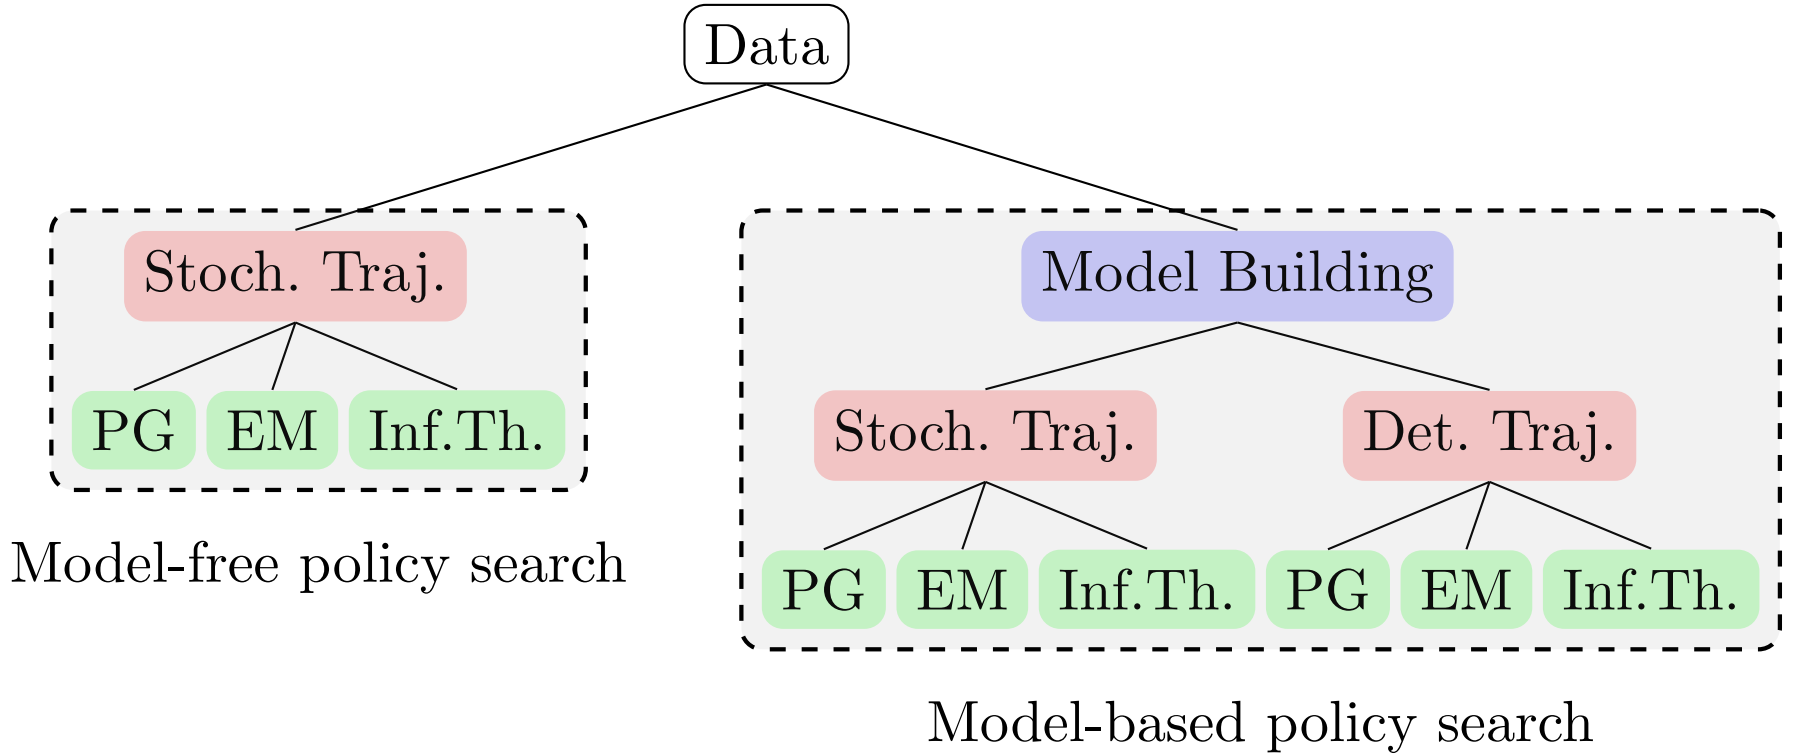
\includegraphics[width=\textwidth,height=\textheight,keepaspectratio]{Images/ps_taxonomy.png}
\caption{A taxonomy of \gls{PS} methods \cite{deisenroth2013survey}} \label{fig:PStaxonomy}
\end{figure}



\section{Policy gradient}
In the context of model-free \gls{PG}, the agent's behaviour is modelled as a differentiable parametric policy $\pi_{\vtheta}:\Sspace\to\Delta(\Aspace)$, independent of time (\emph{stationary}), such that the current action is drawn as $a_h\sim\pi_{\vtheta}(\cdot|s_h)=\pi(\cdot|s_h, \vtheta)$, where $\vtheta\in\Theta\subseteq\Reals^m$ are the policy parameters. The most simple parametrization one could think of is the linear one, where the policy only depends linearly on the policy parameters and the action is drawn deterministically:

\begin{align}
a = \pi_{\vtheta}(s) = \vtheta^T\phi(s),
\end{align}

where $\phi(s)$ can be any differentiable approximation function. In stochastic formulations, typically, a zero-mean Gaussian noise vector is added to $\pi_{\vtheta}(s)$, so that the policy becomes:

\begin{align}
\pi_{\vtheta}(a|s) = \frac{1}{\sqrt{2\pi}\sigma}\exp\left(-\frac{1}{2}\left(\frac{a-\vtheta^T\phi(s)}{\sigma}\right)^2\right).
\end{align}

In some cases, the covariance matrix can be learned as well and the parameters set becomes $\{\mu_{\vtheta}=\vtheta^T\phi(s); \Sigma\}$. In most cases, $\Sigma$ is diagonal, thus easing the complexity of the learning task along with the theoretical analysis. Hence, problem \ref{PSproblem} translates to finding the policy optimal parameters:

\begin{align}
\vtheta^* &= \arg \max_{\vtheta\in\Theta}J(\vtheta).
\end{align}

This new optimization problem can be solved by resorting to gradient ascent on the policy parameters, which is guaranteed to converge to a local optimum at least:

\begin{align}
\vtheta^{h+1} \leftarrow \vtheta^h+\alpha\boldsymbol{G(\vtheta^h)}\nabla_{\vtheta}J(\vtheta),
\end{align}

where $\alpha\geq 0$ is the \emph{learning rate} or \emph{step size}. The quantity $\nabla_{\vtheta}J(\vtheta)$ denotes the \emph{policy gradient} \gls{PG} which gives the name to this method. Its expression is derived in \cite{sutton2000policy}.

\begin{theorem} \label{th:PGtheorem}
\emph{Policy Gradient Theorem} Given a \gls{MDP} $\mathcal{M}$ and a  Markovian stationary stochastic parametric policy $\pi_{\vtheta}$ differentiable \wrt to $\vtheta$ for all state-action pairs $(s,a)\in(\Sspace,\Aspace)$, the gradient of the policy performance is given by:

\begin{align}
\nabla_{\vtheta}J(\vtheta) 
&= \int_{\Sspace}d^{\pi_{\vtheta}}(s)\int_{\Aspace}\nabla_{\vtheta}\pi_{\vtheta}(a|s)Q^{\pi_{\vtheta}}(s,a)dads \nonumber \\
&= \myExpu{s\sim d^{\pi_{\vtheta}}, a\sim \pi_{\vtheta}(\cdot|s)}{\nabla_{\vtheta}\log\pi_{\vtheta}(a|s)Q^{\pi_{\vtheta}}(s,a)}  . \label{eq:PGtheorem}
\end{align}
\end{theorem}

$\pi_{\vtheta}(s)$ is the stationary state distribution induced by policy $\pi_{\vtheta}$, as defined in equation \ref{eq:ssdistribution}. In practical applications it can be inconvenient or impossible to compute the Q-function. One solution is to leverage simple function approximators belonging to the class of \emph{compatible basis functions}, \ie functions of the form $f_{\vomega}=\vomega^{T}\nabla_{\vtheta}\log\pi_{\vtheta}(a|s)$. Such approximators can replace $Q^{\pi_{\vtheta}}(s,a)$ in equation \ref{eq:PGtheorem} for the calculation of the policy gradient as proven in \cite{sutton2000policy}.\\
A second solution that prevent from calculating $Q^{\pi_{\vtheta}}(s,a)$ explicitly is to resort to a trajectory-based reformulation of equation \ref{eq:PGtheorem}. By rephrasing the expected performance under policy $\pi_{\vtheta}$ defined in equation \ref{eq:Jstartstate} as:

\begin{align}
J(\vtheta) = \Exp_{\tau\sim p_{\vtheta}}[\Rew(\tau)], 
\end{align}

where $p_{\vtheta}$ is the distribution over trajectories $\tau\in\mathcal{T}$ induced by the policy $\pi_{\vtheta}$, we can write: 

\begin{align}
\nabla_{\vtheta}J(\vtheta) = \int_{\mathcal{T}}\nabla_{\vtheta}p_{\vtheta}(\tau)\Rew(\tau)d\tau = \myExpu{\tau\sim p_{\vtheta}}{\nabla_{\vtheta}\log p_{\vtheta}(\tau)\Rew(\tau)}
\end{align}

This formulation of the \gls{PG} turns out to be extremely practical. Not only because it prevents from the calculation of the Q-function, but also because it does not require any knowledge about the transition kernel of the \gls{MDP}. In fact, $\log p_{\vtheta}(\tau)$ can be easily derived from the sheer knowledge of the trajectory and definition of the policy:

\begin{align}
\log p_{\vtheta}(\tau) 
&= \nabla_{\vtheta}\log\left( \mu(s_{\tau,0}\prod_{t=0}^{H-1}\pi_{\vtheta}(a_{\tau,h}|s_{\tau,h})\Tran(a_{\tau,h+1}|s_{\tau,h+1}))\right) \\
&= \sum_{t=0}^{H-1}\nabla_{\vtheta}\log\pi_{\vtheta}(a_{\tau,h}|s_{\tau,h}), \; \forall \tau\in\mathcal{T}
\end{align}



%\todol{draw markov reward process example}
%\todol{A MAB is formally equivalent to a one-step Markov Decision Process (MDP), with 3 arms MAB drawing} 
%\begin{center}
%\begin{tikzpicture}[->, >=stealth', auto, semithick, node distance=3cm]
%\tikzstyle{every state}=[fill=white,draw=black,thick,text=black,scale=1]
%\node[state]    (A)                     {$A$};
%\node[state]    (B)[above right of=A]   {$B$};
%\node[state]    (C)[below right of=A]   {$C$};
%\node[state]    (D)[below right of=B]   {$D$};
%\path
%(A) edge[loop left]     node{$p^2$}         (A)
%    edge[bend left]     node{$(1-p)^2$}     (B)
%    edge[bend left,below]      node{$p(1-p)$}      (D)
%    edge[bend right]    node{$p(1-p)$}      (C)
%(B) edge                node{$1$}           (D)
%(C) edge                node{$1$}           (D)
%(D) edge[loop right]    node{$(1-q)^2$}     (D)
%    edge[bend right,right]    node{$q(1-q)$}      (B)
%    edge[bend left]     node{$q(1-q)$}      (C)
%    edge[bend left,above]     node{$q^2$}         (A);
%\node[above=0.5cm] (A){Patch G};
%\draw[red] ($(D)+(-1.5,0)$) ellipse (2cm and 3.5cm)node[yshift=3cm]{Patch H};
%\end{tikzpicture}
%\end{center}

